\documentclass[tikz,border=2mm]{standalone}
\usetikzlibrary{positioning,matrix,arrows.meta}
\usepackage{amssymb}

\begin{document}
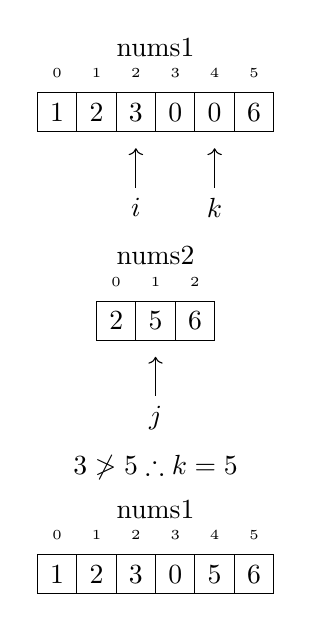
\begin{tikzpicture}[nodes in empty cells,
      nodes={minimum width=0.5cm, minimum height=0.5cm},
      row sep=-\pgflinewidth, column sep=-\pgflinewidth]

      % Current state of nums1 array
      \matrix(vector)[matrix of nodes,
          row 1/.style={nodes={draw=none, minimum width=0.3cm}},
          nodes={draw}]
      {
          \tiny{0} & \tiny{1} & \tiny{2} & \tiny{3} & \tiny{4} & \tiny{5} \\
          ${1}$ & ${2}$ & ${3}$ & ${0}$ & ${0}$ & ${6}$\\
      };

      % Label nums1 array
      \node[above=-3mm of vector] {nums1};

      % Draw i and k arrows under nums1
      \draw[<-] ([yshift=-2mm]vector-2-5.south) -- ++(0,-0.5) node[below] {$k$};
      \draw[<-] ([yshift=-2mm]vector-2-3.south) -- ++(0,-0.5) node[below] {$i$};

      % Current state of nums2 array
      \matrix(vector2)[matrix of nodes, below=14mm of vector,
          row 1/.style={nodes={draw=none, minimum width=0.3cm}},
          nodes={draw}]
      {
          \tiny{0} & \tiny{1} & \tiny{2} \\
          ${2}$ & ${5}$ & ${6}$ \\
      };

      % Label nums2 array
      \node[above=-3mm of vector2] {nums2};

      % Draw j arrow under nums2
      \draw[<-] ([yshift=-2mm]vector2-2-2.south) -- ++(0,-0.5) node[below] {$j$};

      % Show comparison result
      \node(comparison)[below=12mm of vector2] {$3 \ngtr 5 \therefore k = 5 $};

      % Updated state of nums1 array
      \matrix(vector3)[matrix of nodes, below=2mm of comparison,
          row 1/.style={nodes={draw=none, minimum width=0.3cm}},
          nodes={draw}]
      {
          \tiny{0} & \tiny{1} & \tiny{2} & \tiny{3} & \tiny{4} & \tiny{5} \\
          ${1}$ & ${2}$ & ${3}$ & ${0}$ & ${5}$ & ${6}$\\
      };

      % Label updated nums1 array
      \node[above=-3mm of vector3] {nums1};



\end{tikzpicture}
\end{document}
